%% Developing a solution for multimedia home networking chapter
%% author Liu Peng

To fulfill the need for interoperability among devices in home networking,
Tuxera Inc. started a project named Streambels (later renamed as AllConnect).
The project aims to solve the interoperability issue in multimedia home networking
by making a universal solution that can connect all available devices at home
and allow them to work together regardless of their protocol. During this
project, I worked as a major developer, helping with the design and
implementation of this application, and ensure the interoperability with DLNA
standard.

Most devices at home are embedded solutions and have their own firmwares; it is
difficult to update or even impossible to upgrade the software running on these
devices. On the other hand, most home network users are not knowledgeable
enough to manually set up the more advanced network features to achieve a
certain degree of device interoperability. In addition, most of these network
infrastructures are not designed to be easily configured. Due to these reasons,
building interoperability among different devices through a mobile device seems
to be the most straightforward solution. Mobile devices can serve as a quite
flexible and programmable portal for home networking.  Other advantages of
mobile devices include their great processing power, networking capabilities,
and their wide adoption and availability. Through the available platforms and
tools, a mobile application could possibly be developed to control all
multimedia streaming data flows and act as a personal access portal for home
networking.

After a year of development, the team have created an Android
application\footnote{\url{http://allconnectapp.com/}} that can control and
connect every known type of multimedia device at home. I tested and fixed the
interoperability with many DLNA receivers and media servers which are
manufactured by different kinds of manufacturers. This effort has enabled the
application to work with most devices in a common home networking environment. I
also implemented the streaming server and streaming proxy, which served as the
source of streaming. Encouragingly, the number of the application users has
grown to nearly one million so far, providing strong proof of the effectiveness
of this solution.

This chapter describes the solution we developed for multimedia home networking.
Section \ref{3_1} proposes the solution and introduces the overall architecture
of the proposed solution. Section \ref{3_2} describes the detailed
implementation aspects of our solution. Section \ref{3_3} describes the user
interface and user experience design. Section \ref{3_4} discusses the features
of our solution. Section \ref{3_5} discusses the possibility to extend our
solution to other content sources. Section \ref{3_6} describes the methodology
of software testing and how our solution is tested before releasing to market.
Finally, Section \ref{3_7} introduces the methodology to evaluate our solution.

\subsection{Architecture overview\label{3_1}}
In order to solve the multimedia home networking interoperability problem, the
system should be designed to control media playback sessions. Consequently,
content navigation, managing the receiver device, and media playback should be
the most important three components. In the solution, the system architecture
consists of three major parts: the device discovery, content management and streaming.

The discovery component is responsible for device discovery. As discussed
in \ref{upnp}, UPnP/DLNA devices and DIAL devices utilize Simple Service Discovery
Protocol (SSDP) for device discovery. An application firstly sends an M-Search
request over UDP to the IPv4 multicast address 239.255.255.250 and UDP port
1900. Then, the application listens to other devices' responses. A DIAL device
will return a response with an Application URL header, while the UPnP/DLNA
devices will return a message with an XML body, which provides detailed service
URLs and description URLs. Instead of using the SSDP discovery, Apple products,
by comparison, use Multicast DNS for device and service discovery. Obviously,
in order to support the three types of devices, namely the UPnP/DLNA devices,
the DIAL devices and the Apple Airplay devices, we need to integrate these two
mentioned discovery mechanisms, namely, the SSDP mechanism and the Multicast
DNS mechanism, into our solution.

The content management component is responsible for organizing and navigating
in multimedia contents that can be discovered in the home network. In our
solution, these content sources include both the local storage of smart phones
and DLNA digital media servers that are connected to the home network. As long
as the discovered device belongs to the three device types that this solution
support, its content could be streamed using the application solution.

The streaming component is responsible for streaming multimedia content to the
selected multimedia receivers, such as TVs, wireless speakers, set-top boxes and so on. In a typical home networking environment, DLNA, AirPlay video/photo, and Chromecast all use HTTP streaming. The only exception, AirPlay music, uses Remote Audio Output Protocol (RAOP). Because of this, two types of media servers were integrated inside the application solution. With the application, the built-in RAOP server would handle the AirPlay music streaming, and the built-in HTTP media server would handle streaming of all other types.

\subsection{Implementation\label{3_2}}
Since the application is built upon the Android platform, we conducted research
on the Android system architecture and the Android Software Development Kit
(SDK). Thankfully, the Android SDK provides many useful Application Programming
Interfaces (APIs) and grants crucial permissions to access necessary services
and hardware features, such as the permission to access the Internet , the
permission to access the WiFi device state change, the permission to allow WiFi
multicast and  the permission to read phone storage. The programming language
used in developing our Android Application is Java. However, some CPU-intensive
works, such as transcoding, have to be implemented in C, and then embedded to
the application using the Android Native Development Kit (NDK).

Since Apple has not provided its official specification for AirPlay, our
implementation for supporting AirPlay is mostly written under unofficial
guidelines \cite{AirPlay-spec}. However, Apple has provided its official
Multicast DNS (mDNS) implementation in C
\footnote{\url{https://developer.apple.com/bonjour/index.html}}. Thus, this
piece of code is reused and compiled as a shared native library. Similar with
the Airplay support, the support for Remote Audio Output Protocol (RAOP) is
also implemented under unofficial guidelines.
To be specific, the RAOP supporting component includes a UDP server and a TCP
control channel.

With Tuxera being a member of DLNA , we are able to access the detailed specifications and test tools for DLNA. Moreover,  there are a lot of open source UPnP/DLNA
 libraries available since DLNA is now a popular standard. Specifically, in our
 implementation, we uses a library called "cling" \cite{cling}
 \footnote{\url{http://4thline.org/projects/cling/}}, which provides minimal
 implementation of UPnP device discovery, description information parsing, and basic message handling. By extending "cling" \cite{cling}, we are able to provide media formats compatibility across different devices.

Google has officially provided the Chromecast SDK for different mobile platforms, which enables us to  implement the Chromecast integration with ease. In the Streambels project, the Chromecast integration is built upon the Chromecast API.

When it comes to media server implementation, according to the DLNA guidelines,
certain additional headers need to be implemented in the stream. This
requires the HTTP server to possess the functionality to add DLNA specific
headers. Another requirement is that the "Seek" action needs to be supported on the server side. To support "Seek", byte based seeking operations are enabled in our implementation.

For receivers who do not use the DLNA standard, a basic file server with byte
range support will be sufficient to do the work.

In addition, in order to serve media for all the receivers from both online and
local storage, a separate media proxy also needs to be implemented
\cite{ipv6} \cite{DLNA_proxy2}.

After investigating and comparing multiple server implementations on Android, we
concluded that NanoHTTPD\footnote{\url{http://nanohttpd.com/}} is the ideal
choice for our solution, because NanoHTTPD is easy to use, Apache licensed,
very tiny and efficient. Since NanoHTTPD is minimally implemented, it is also
easy to be modified and extended. With NanoHTTPD , additional headers can be
easily added to make the server implementation compatible with DLNA receivers.
Besides, a proxy is also easy to integrate with  NanoHTTPD.

Taking all these technical details into consideration, we devised a simplified
architecture for our implementation, which is shown in Figure \ref{chart3}.

\begin{figure}[htb]
\centering 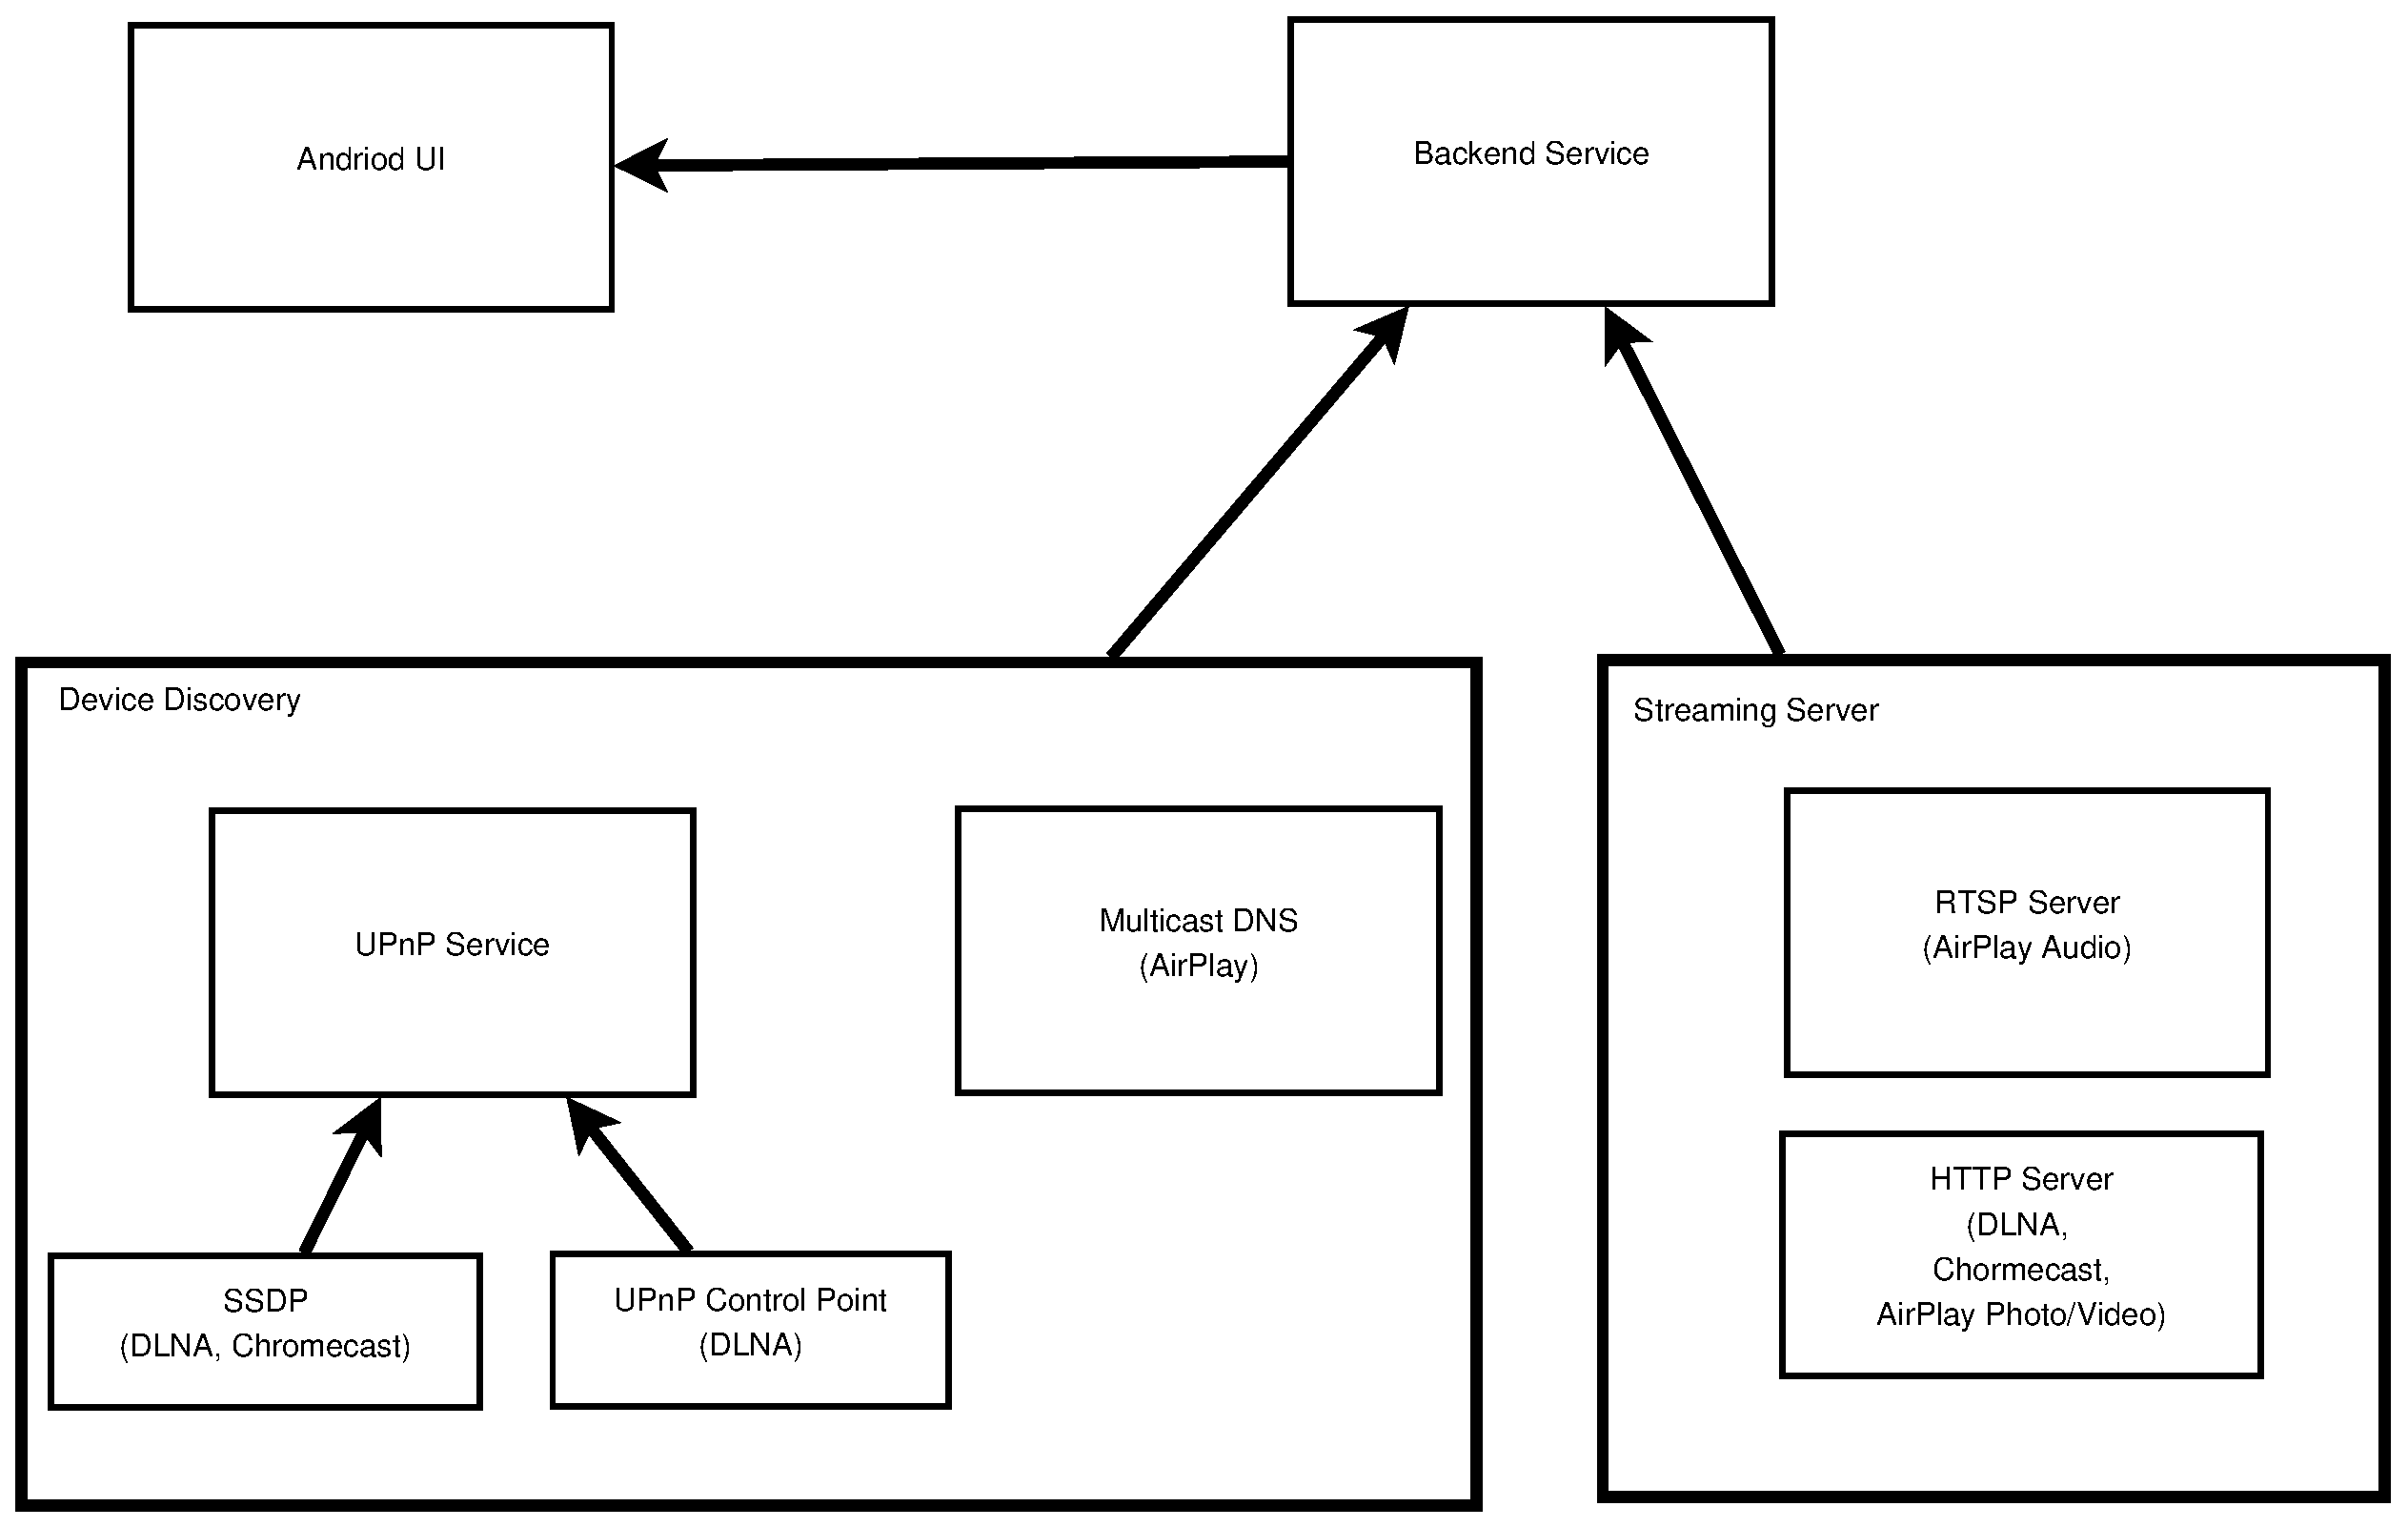
\includegraphics[height=9cm]{charts/chart3}
\caption{Simplified application architecture\label{chart3}}
\end{figure}

When streaming content, the data flow is different for different scenarios.
Figure \ref{chart4} shows the three use scenarios and their corresponding data
flows:

If the content is stored in a mobile phone, a streaming server in the
application will be used to stream the content from the mobile device to the
selected receiver.

In contrast, if the content is located on the Internet and the receiver is a
DLNA Media Renderer, a proxy will be needed. To be specific, the proxy will
first download the resource stream and then add certain headers required by the
DLNA specification. After that, the proxy streams the modified content to the
selected DLNA Media Renderer.

Finally, if the streamed content locates in a DLNA Digital Media Server, then
the source can be used directly by all receivers. In this case, the streaming
proceeds directly from the media server to receivers. Our application, in this
scenario, will only be used as a control point and do not really participate in
the media transmission, as shown in Figure \ref{chart4}.

\begin{figure}[htb]
\centering 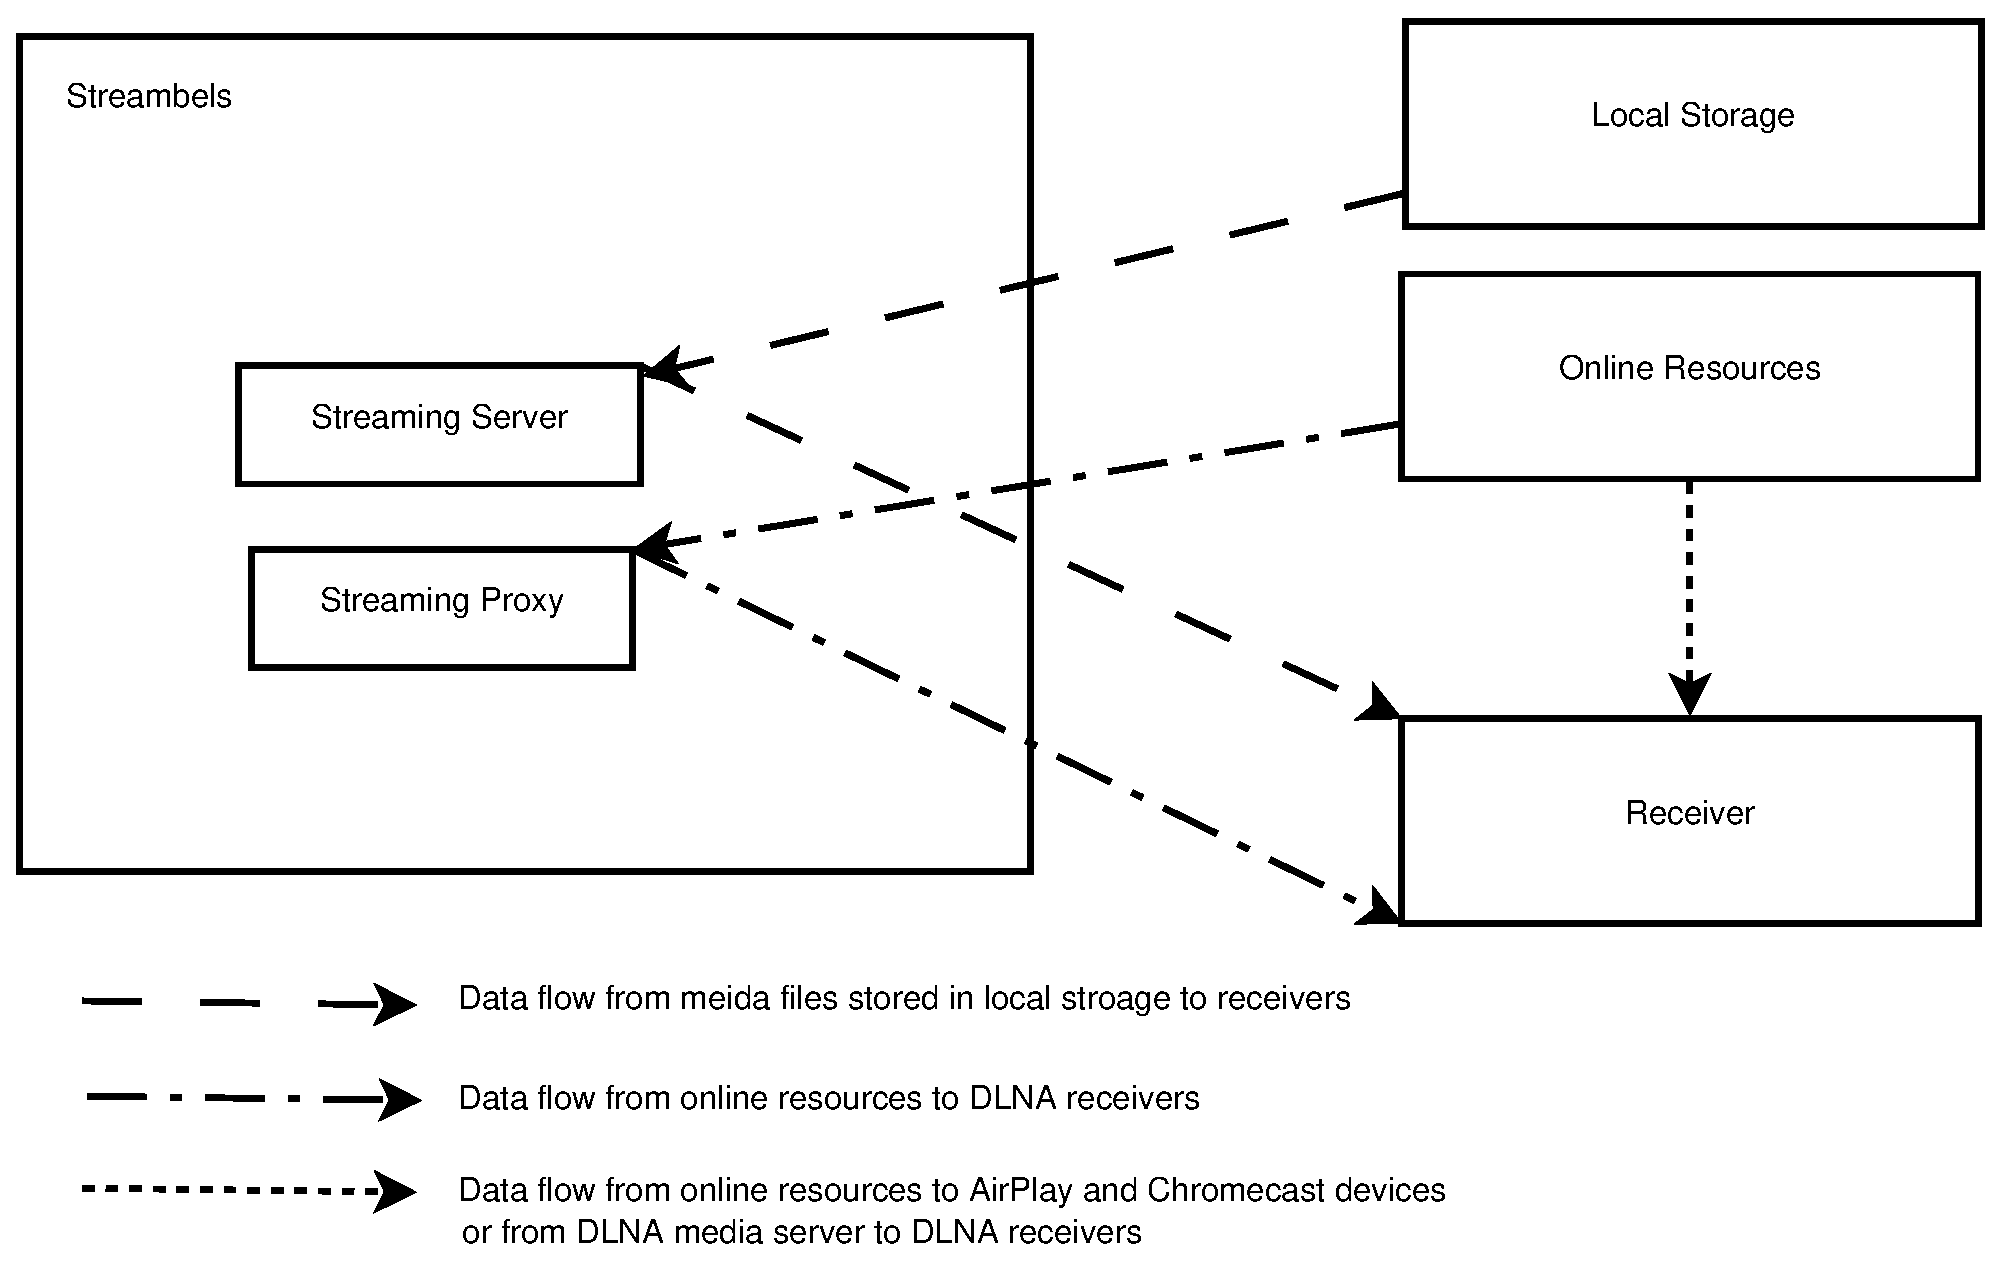
\includegraphics[height=9cm]{charts/data_flow}
\caption{Simplified data flow \label{chart4}}
\end{figure}

\subsection{User Experience design\label{3_3}}
In terms of User Interface (UI) and User Experience (UX), the application should
be simple enough to use. Users should be able to locate the media, browse
content on different sources, and follow the data flow between devices without
any difficulty. The control of different devices should also be intuitive so
that the inter-operation between different devices can be seamless.

A multimedia home networking solution should be content centric so that the user
can easily navigate through different sources. The application is designed
similar to a multimedia player. A cast button is added at the top of the
application to make it easier to select cast devices. The content is
categorized into 4 sections: music, video, photo and online sources. In
Android, since the system provides share intent method for inter-activity
communication, an interface is also made to manage share intents from other
activities, which enables streaming from other on-line content providers. The
selected receiver is designed to be visible to the user from everywhere inside
the application.

Bearing all these considerations in mind, the final appearance of the application becomes simple and effective. Figure \ref{chart5} shows the final design of our application.

\begin{figure}[htb]
\centering 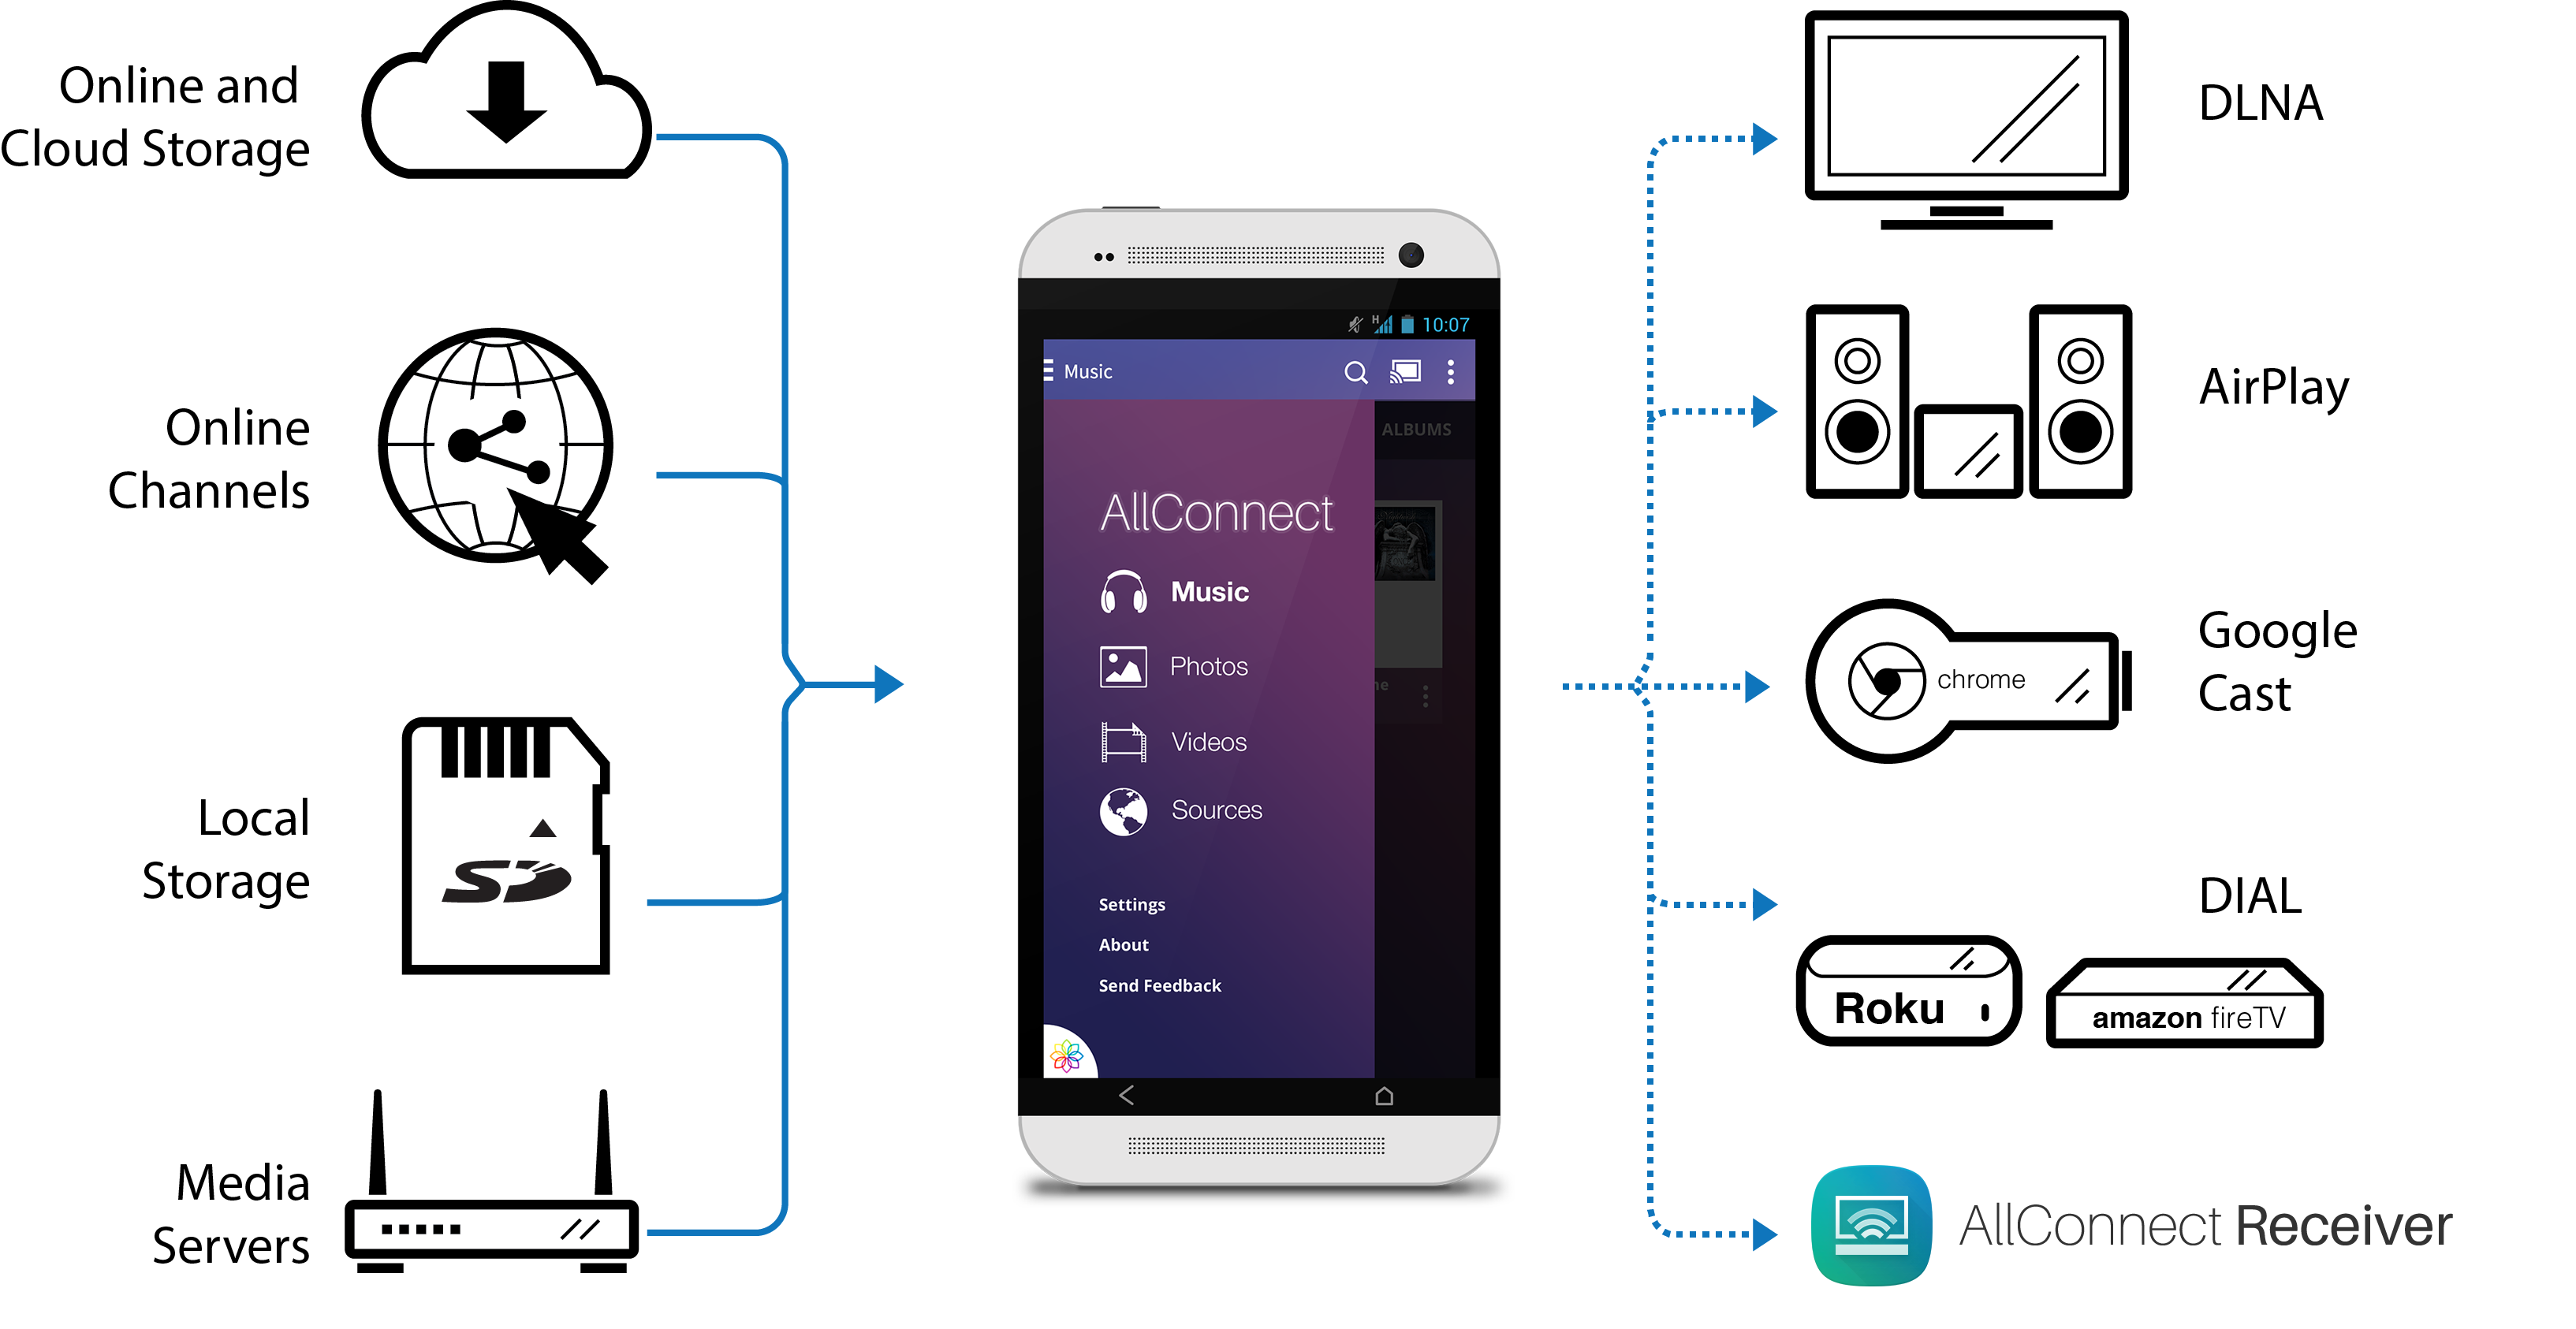
\includegraphics[height=8cm]{charts/allconnect-app}
\caption{Application UX design \label{chart5}}
\end{figure}

\subsection{Features\label{3_4}}
The Android application we have developed can handle most multimedia devices in typical home networking. It also provides various features, making it a powerful and universal solution for multimedia home networking.

Firstly, the application itself is a multimedia player. Both the media stored locally on the phone storage and the media located in the DLNA media servers can be browsed and played locally on the phone.

Secondly, the application is fully compatible with AirPlay, DLNA, Chromecast and FireTV receiver devices. All devices can be discovered as renderer devices.

Thirdly and most importantly, the application enables the DLNA media server to
work together with all kind of receivers regardless of the protocol used. The
app serves as a bridge for different multimedia receivers and media sources.

Lastly, YouTube and other on-line channels like Vimeo and Facebook are
supported as available media sources. The content can be streamed, regardless
of the protocol, to all supported receivers that are connected to the home
network.

\subsection{Extensibility\label{3_5}}
Streambels has embedded a media streaming server for local files and a streaming proxy for bridging the gap between online resources and home networking. By using a built-in proxy, Streambels is able to share on-line resources from the Internet to devices in home networking environment.

New service providers and content providers can integrate home networking
support into their products easily by just sending formatted intent to our
application following our guidelines. The proxy will automatically bridge the
gap between the Internet and the home network.

The proxy system provides great extensibility and makes it possible to connect home networking to Internet or Cloud Services.

In the future we could also develop a Software Development Kit (SDK) to grant the availability of our technology, enabling other application builders to directly use our home-networking solutions.
\subsection{Test methodology\label{3_6}}
Software testing is extremely important for a modern IT project. Buggy
implementation may kill the product in the very beginning since it can badly
undermine the user experience. Through testing we could assure the performance
and stability of our product. Thus, before the final release to the Google Play
store, the application was thoroughly tested.

These tests included unit test, integration test and functional test.
Unit tests were conducted while coding the application. When each class was
finished, unit tests would be written for each method. We also set up an
continuous integration server so that each time we commit anything to the git
repository, the full set of unit tests would be executed. If there was any
failure in the unit tests, the developer would be immediately notified.
Integration tests were done for we ensuring that each function module works
together with other modules in the system. Lastly, we listed all the possible
use cases on paper and prepared a huge media base containing all kind of
media files. With all these preparations ready, manual tests were conducted
before the app was finally released in the market.

\subsection{Evaluation methodology\label{3_7}}
This section discusses the methodology to evaluate our application. Section
\ref{3_7_1} describes the experiments to evaluate the performance of
the Streambels application. Section \ref{3_7_2} introduces the methodology we
use to collect user activities and user feedbacks.

\subsubsection{Experimental setup\label{3_7_1}}
The test environment is set up as in Figure \ref{setup}. The XBMC
media receiver is running on MacBook A and Streambels is running on a rooted
Android phone B. Both A and B are connected to a router C using the 802.11 ac
wireless interface. \\
\begin{figure}[htb]
\centering 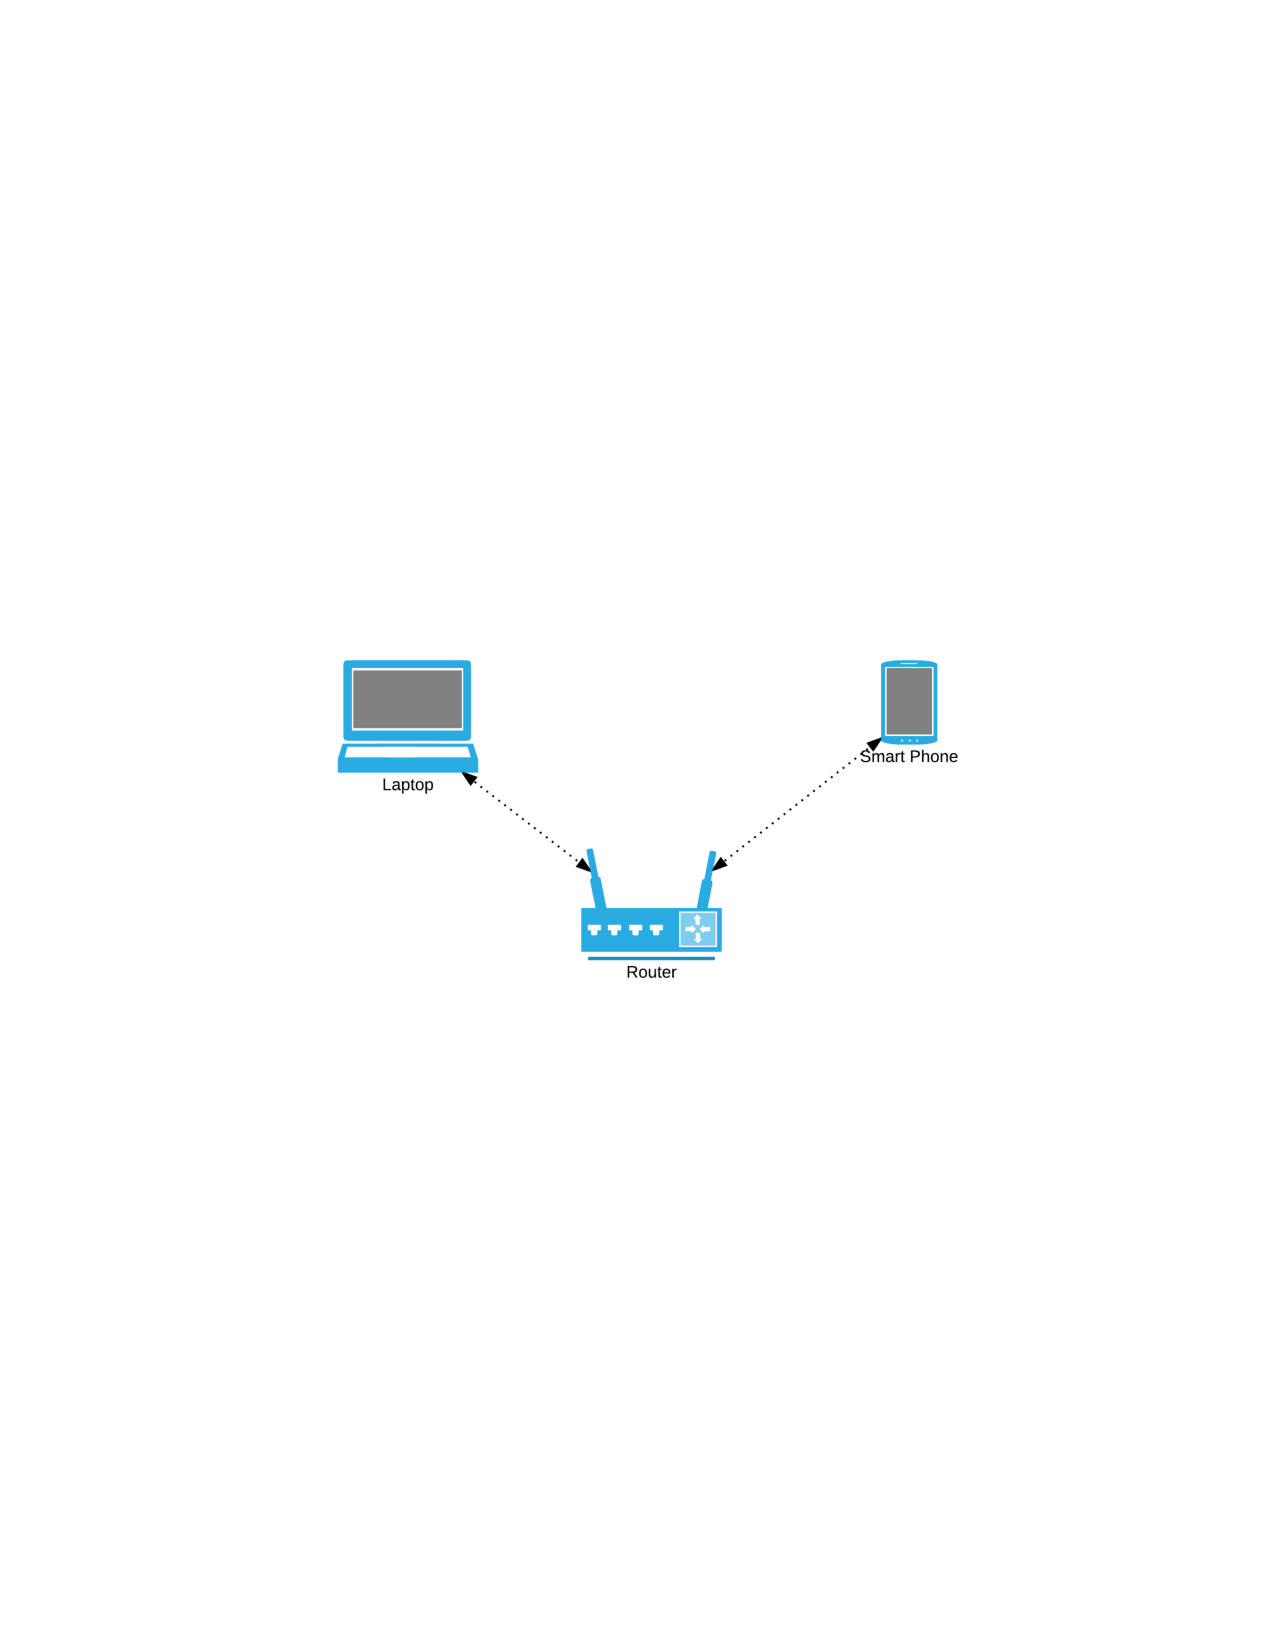
\includegraphics[height=7cm]{charts/experiment_setup}
\caption{Experiment setup \label{setup}}
\end{figure}
With the support of both AirPlay and DLNA protocols, XBMC is an open source media center software that can run on different platforms. It is a popular software solution that is widely used in home networks, which has been ported to different platforms including Raspberry PI.

Network Link Conditioner is an application provided by Xcode that runs on Mac to emulate network conditions, such as packet loss, network delay and bandwidth variations. By changing the configurations, different network conditions can be set to determine the boundary network conditions.

Wireshark is an useful developer tool to capture and analyze network traffic.
It can be installed on both the sender and receiver side. However, it can only
be installed on rooted Android phones to gain the access to network interface
on Android. In our setup, Wireshark is installed on MacBook because we need to
adjust network condition on the receiver side and there might be packet loss
since some solutions may use the UDP protocol.

When the test starts, the same content will be streamed to receivers using two different standards, AirPlay and DLNA. The same test will be run several times to get the average statistics. Different parameters will also be tested by using different network condition configurations.
Bandwidth and packet loss are taken into consideration when conducting the
tests.
\subsubsection{User study and feedback collection\label{3_7_2}}
Since the product is targeted to the Android market and is directly used by end
users, user feedback is really important to us for improving the product
continuously. Email is used for normal communication between the user and our
support. A submission window is built inside the application, so that users can
easily send feedback to us directly by Email.

There is no perfect program, crashes sometimes happen. Thanks to Google, all crash reports are collected and displayed inside developer console. This makes it a lot easier to track and debug our application.

Inside Streambels, we also integrated Google's Analytics API. The API provided
great convenience for us to collect the number of users and sessions every day.
Other information such as operating system version, application version and the
number of active users as well as user feedbacks, have helped us to gain more
insight in our application and the market response, making it easier for us to
improve the application and do better marketing.

It is also interesting to see what kind of technologies are most used in their
daily life. With the Google analytics SDK, we could trigger events when users
select their receivers. After months of monitoring and statistics collection,
we have been able to figure out the most popular standards and most popular
online channels.

This valuable information will in turn help our decision making on how we should
improve our application. Some of these result will be discussed in Chapter
\ref{chapter4}.
